\documentclass[tikz,border=8pt]{standalone}
\usepackage{amsmath,amssymb}
\usetikzlibrary{arrows.meta,automata,positioning,quotes}
\begin{document}
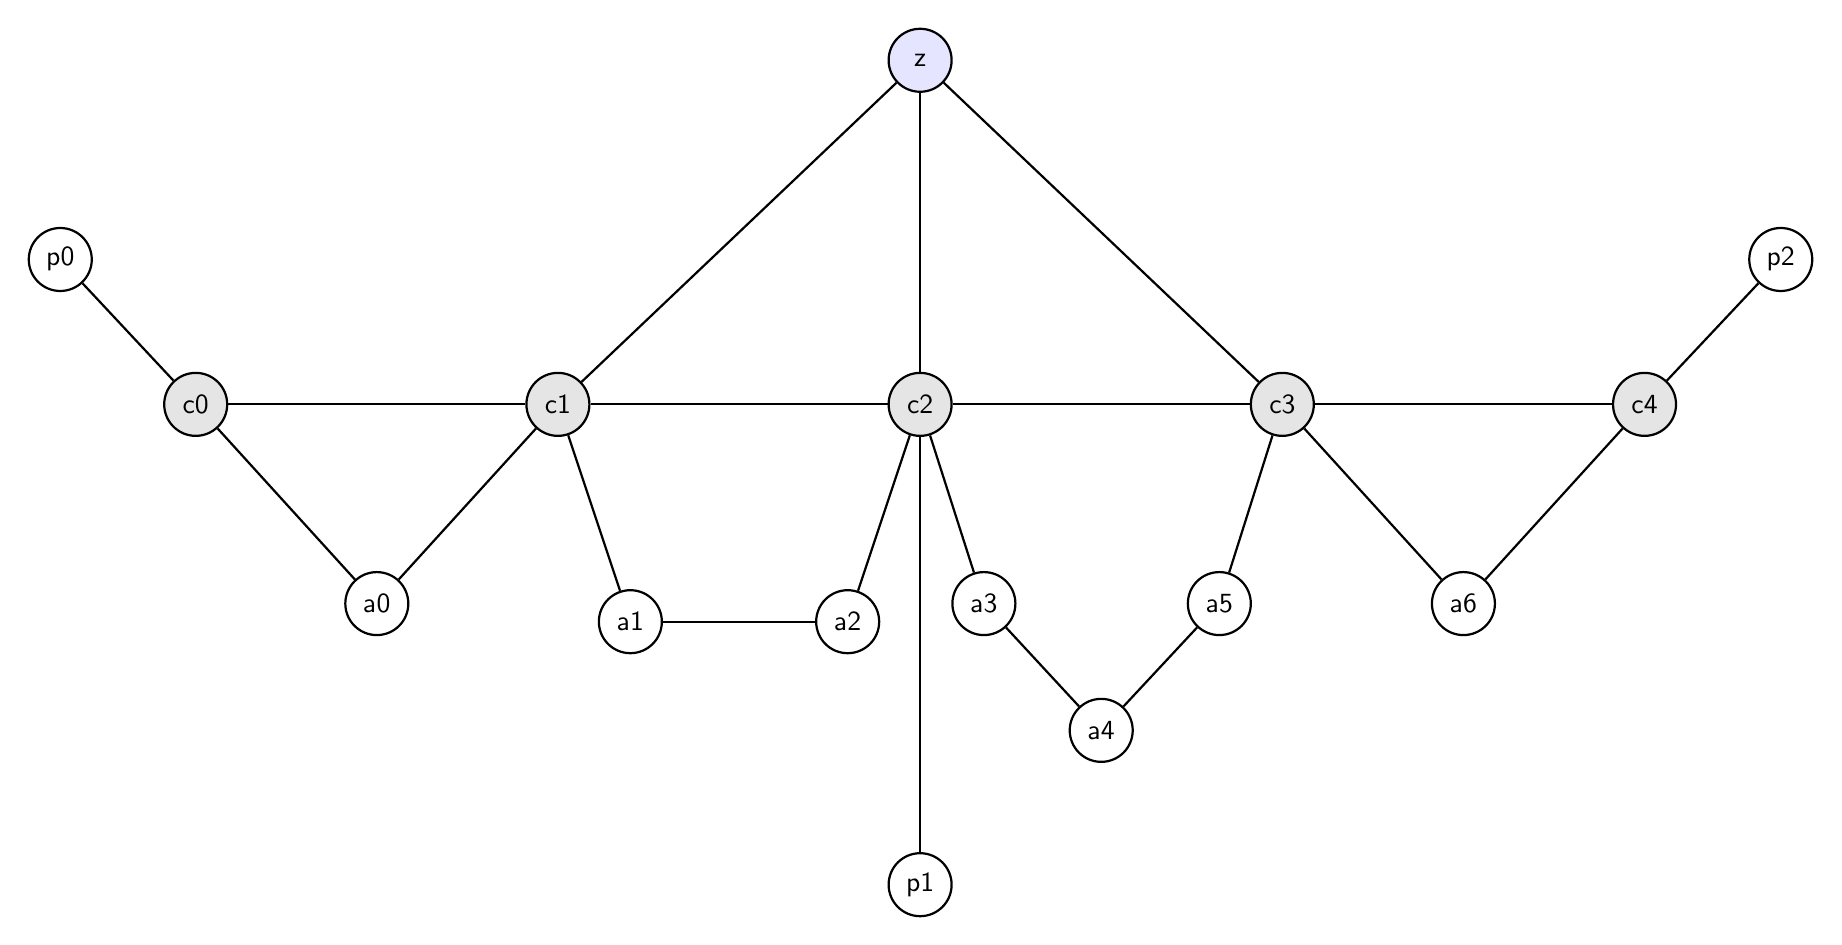
\begin{tikzpicture}[x=1cm,y=1cm]
\tikzset{
  graphnode/.style={circle,draw,thick,minimum size=8mm,inner sep=1pt,font=\sffamily},
  directed/.style={-{Stealth[length=2.4mm]},thick},
  undirected/.style={thick}
}
\node[graphnode,fill=black!10] (n_c0) at (-1.22,0.15) {c0};
\node[graphnode,fill=black!10] (n_c1) at (3.38,0.15) {c1};
\node[graphnode,fill=black!10] (n_c2) at (7.98,0.15) {c2};
\node[graphnode,fill=black!10] (n_c3) at (12.58,0.15) {c3};
\node[graphnode,fill=black!10] (n_c4) at (17.18,0.15) {c4};
\node[graphnode] (n_a0) at (1.08,-2.38) {a0};
\node[graphnode] (n_a1) at (4.30,-2.61) {a1};
\node[graphnode] (n_a2) at (7.06,-2.61) {a2};
\node[graphnode] (n_a3) at (8.79,-2.38) {a3};
\node[graphnode] (n_a4) at (10.28,-3.99) {a4};
\node[graphnode] (n_a5) at (11.78,-2.38) {a5};
\node[graphnode] (n_a6) at (14.88,-2.38) {a6};
\node[graphnode] (n_p0) at (-2.94,1.99) {p0};
\node[graphnode] (n_p1) at (7.98,-5.95) {p1};
\node[graphnode] (n_p2) at (18.91,1.99) {p2};
\node[graphnode,fill=blue!10] (n_z) at (7.98,4.52) {z};
\draw[undirected] (n_c0) -- (n_c1);
\draw[undirected] (n_c1) -- (n_c2);
\draw[undirected] (n_c2) -- (n_c3);
\draw[undirected] (n_c3) -- (n_c4);
\draw[undirected] (n_c0) -- (n_a0);
\draw[undirected] (n_a0) -- (n_c1);
\draw[undirected] (n_c1) -- (n_a1);
\draw[undirected] (n_a1) -- (n_a2);
\draw[undirected] (n_a2) -- (n_c2);
\draw[undirected] (n_c2) -- (n_a3);
\draw[undirected] (n_a3) -- (n_a4);
\draw[undirected] (n_a4) -- (n_a5);
\draw[undirected] (n_a5) -- (n_c3);
\draw[undirected] (n_c3) -- (n_a6);
\draw[undirected] (n_a6) -- (n_c4);
\draw[undirected] (n_c0) -- (n_p0);
\draw[undirected] (n_c2) -- (n_p1);
\draw[undirected] (n_c4) -- (n_p2);
\draw[undirected] (n_z) -- (n_c1);
\draw[undirected] (n_z) -- (n_c2);
\draw[undirected] (n_z) -- (n_c3);
\end{tikzpicture}
\end{document}
